\documentclass{article}

\usepackage{siunitx}
\usepackage{tikz}
\newlength\imagewidth           % needed for scalebars
\newlength\imagescale           % ditto
\newcommand{\imsize}{\linewidth}
\begin{document}
\begin{figure}
	\centering
	\pgfmathsetlength{\imagewidth}{\imsize}%
	\pgfmathsetlength{\imagescale}{\imagewidth/1500}%
	\def\x{927}%
	\def\y{800}% scalebar-y at 90% of height of y=1715px
	\begin{tikzpicture}[x=\imagescale,y=-\imagescale]
		\node[anchor=north west,inner sep=0pt,outer sep=0pt] at (0,0) {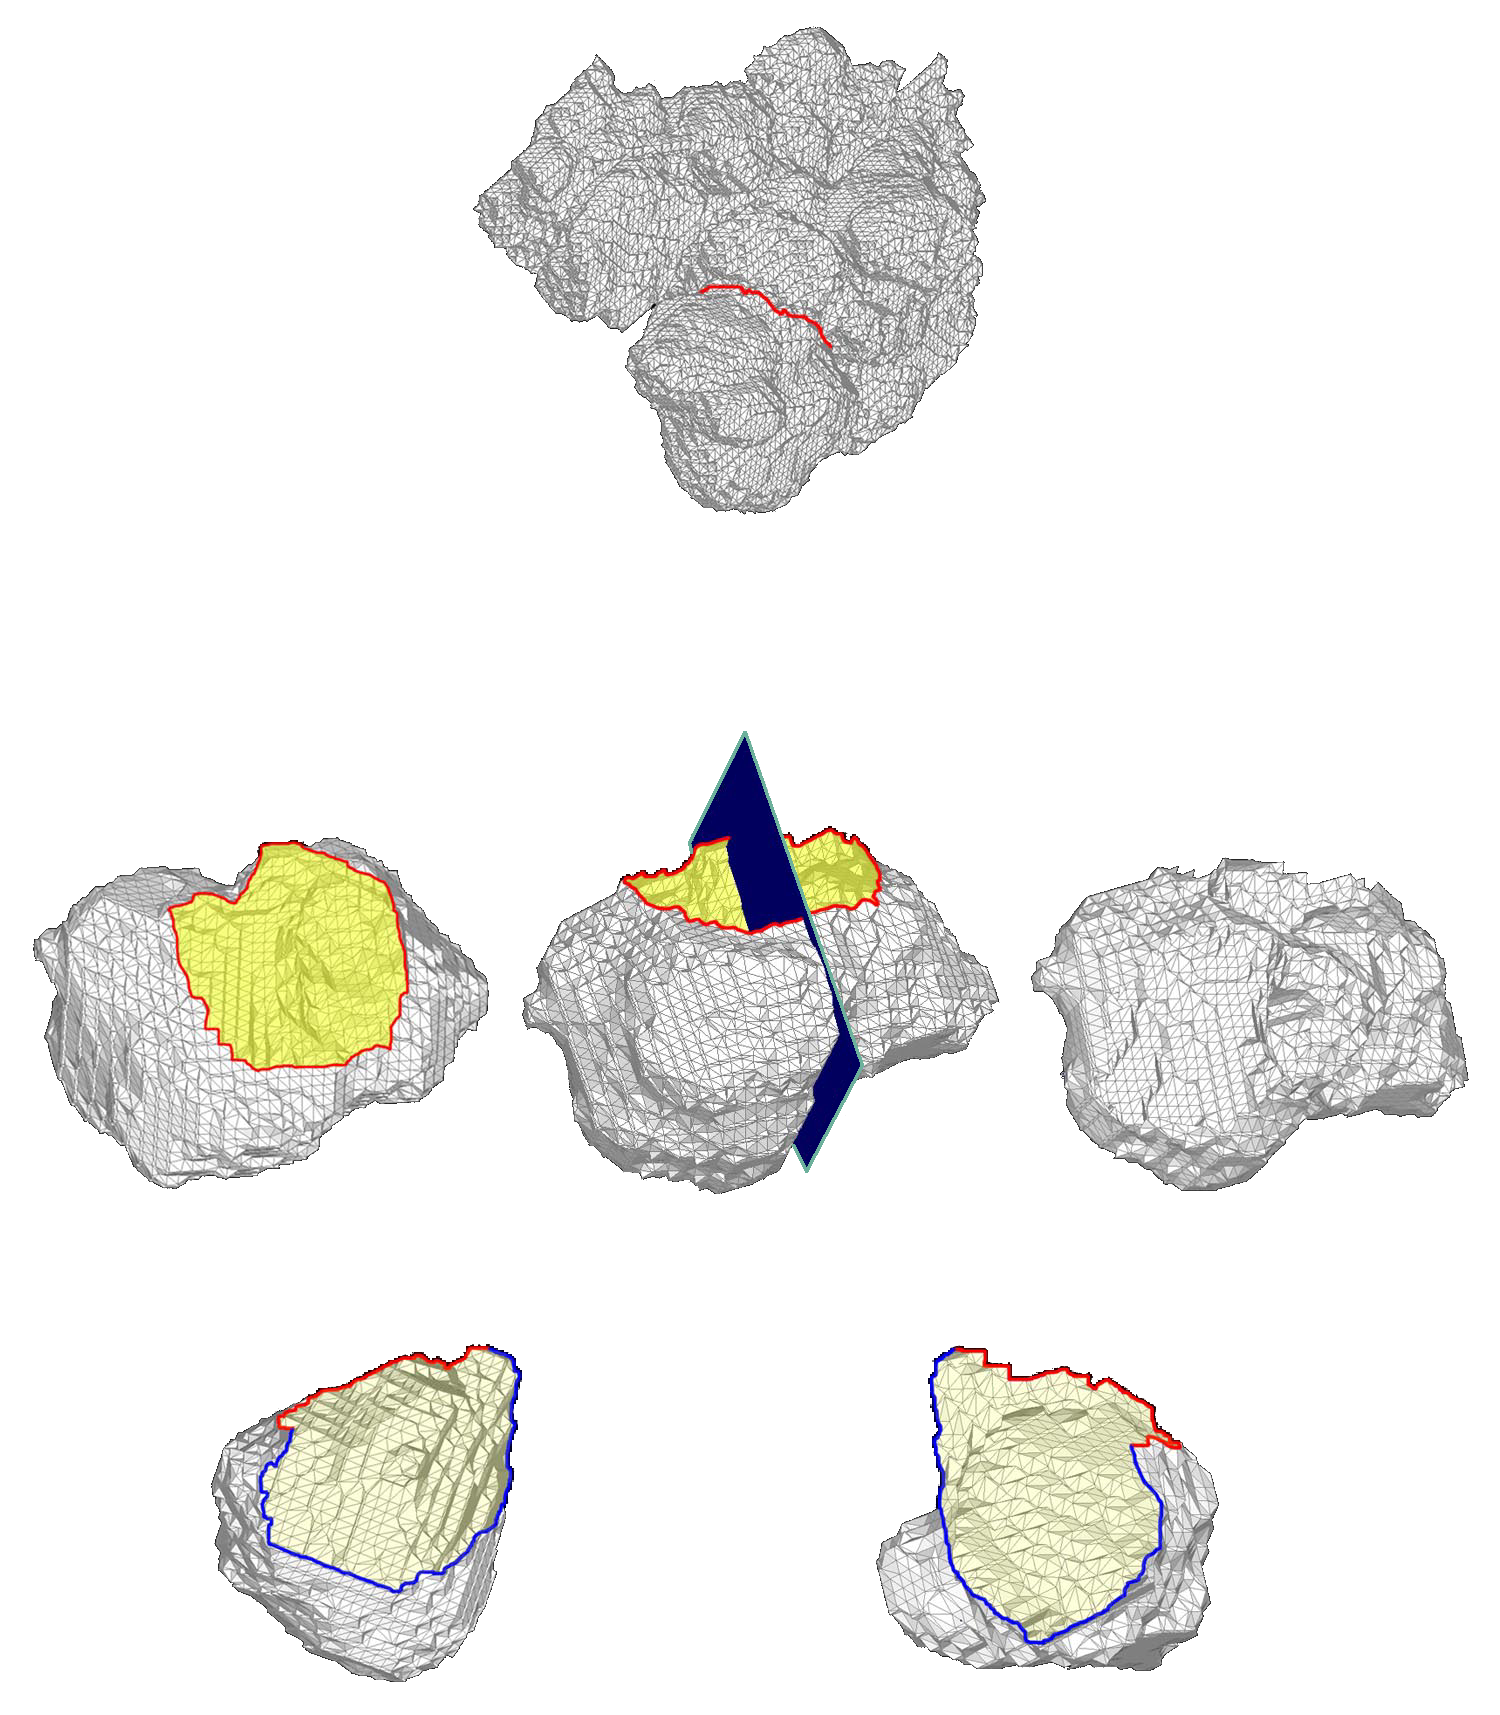
\includegraphics[width=\imagewidth]{Tsuda-10_edit}};
		% 95px = 0.01mm > 100px = 11um > 4752px = 500um, 950px = 100um
		%\draw[red,|-|,thick] (881,1100) -- (976,1100) node [sloped,midway,above] {\SI{0.01}{\milli\meter} (100px)};
		\draw[|-|,thick] (\x-47.5,\y) -- (\x+95,\y) node [midway, above] {\SI{10}{\micro\meter}};
		\draw[->,thick] (750,540) -- (750,690);
		\def\a{106.06601717798212866012665431573}
		\draw[->,thick] (825,1220) -- (825+\a,1220+\a);
		\draw[->,thick] (675,1220) -- (675-\a,1220+\a);
	\end{tikzpicture}%
	\caption{}
	\label{fig:alveolus}
\end{figure}
\end{document}